%\appendix

\chapter{Grouping Model Network}
\label{sec:appendix}
\chaptermark{Grouping Model Network}

\section{Details of model implementation}
\label{sec:appendix_eq}

One pixel in our model input represents the typical size of the receptive
field for 
a V1
edge cell (which at eccentricity 5 $\deg$ is about 0.7
$\deg$, Chen {\em et al}. 2014).  The simulated visual field is
assumed to be homogeneous
(\ie, we neglect the influence of the cortical magnification factor).  
To avoid unbalanced inputs near the
boundaries of the visual field we use periodic boundary
conditions. Each neuronal unit in the model represents multiple
neurons with overlapping receptive fields and similar tuning.  It is
referred to as a ``neuron'' in the following and it is represented by
an ordinary differential equation, eq.~1.  For all examples the system
is simulated for 0.5s and an equilibrium is reached within a few tens
or about hundred ms.  A typical simulation of a visual field of
$64\times 64$ units consists of 30,528 coupled ordinary differential
equations which are solved using a fourth-order Runge-Kutta  algorithm
in MATLAB.

Each neuron is characterized by its spatial location, its type (edge
cell, object grouping cell, \etc) and one additional property, as
follows. E cells are indexed by the angle of their preferred
orientation: $0$, $\pi/4$, $\pi/2$, and $3\pi/4$
(all angles relative to the horizontal). 
B cells are indexed
by the angle of their preferred side of figure: right, $0$; upper
right, $\pi/4$; up, $\pi/2$; upper left, $3\pi/4$; left, $\pi$; lower
left, $5\pi/4$; down, $3\pi/2$; lower right, $7\pi/4$. 
Note that the preferred side of a 
B~cell
 is always orthogonal to its preferred orientation. Contour
grouping cells are indexed by their preferred orientation ($0$,
$\pi/4$, $\pi/2$, and $3\pi/4$), while object grouping neurons are
selective for annuli of a preferred radius.
As discussed earlier, we only use one preferred radius in this model,
which we chose as corresponding to 16 pixels in the input layer.
The network receives two types
of inputs. A binary edge map activates E~cells, taking value 1 if an
edge of that orientation is present
at this location in the image and (-1)
otherwise. Finally, an attentional field stimulates grouping cells,
with maximal strength of 0.07. This value is listed in
Table~\ref{partable}, as are those of all other model parameters.

In the following, we define the anatomical connection patterns between
all neuronal populations in our model. Obviously, this defines the
receptive (and projective) fields of all model neurons. At the input
level, edge cells ($E$ population)  receive 
one-to-one
connections from input units
($IN$ population) of the respective preferred
orientations $o_i$ at 
position $(x,y)$,
resulting in
a connectivity weight distribution as follows,
\begin{align}
	WIN^{o_1}_{x,y}E^{o_2}_{x,y}=
	\begin{cases}
	intoe_w \:\;&if\;o_1 = o_2\\\nonumber
	-1\;&otherwise
	\end{cases}\\
\end{align}
where the weight of the input to edge cell connections, $intoe_w$ is a
scaling parameter, and its value is set to 1.  Changing it does not
produce different activation patterns in the network but rather scales
up all activities.

The connections from edge cells 
to inhibitory IE cells are two-dimensional isotropic Gaussians: 

\begin{align}
	&WE_{x_1,y_1}IE_{x_2,y_2}=N_{etoie}\: \exp\left(-\frac{(x_1-x_2)^2}{2\: etoie_{sd}^2}-\frac{(y_1-y_2)^2}{2\: etoie_{sd}^2}\right)\
\end{align}
where the normalization coefficient $N_{etoie}$ is determined from:
\begin{align}
	etoie_w = \sum^{24}_{i,j=-24} WE_{x,y}IE_{x+i,y+j}
\label{eq:normalizationetoie}
\end{align}

The weight of the edge to IE connections $etoie_w$ is set to 8. The standard deviation of the lateral connections,
$etoie_{sd}$ was chosen to be eight times the size of the edge cells'
receptive field size. For simplicity, all lateral connections in V1
are assumed to have the same standard deviation.
The upper limit in the sum of eq.~\ref{eq:normalizationetoie} is where
we truncate the Gaussian distribution used to define the
connectivities, at three times its standard deviation (8), equal to 24
times the size of a V1 RF.

IE cells are not orientation selective, and inhibit all edge cells in
their neighborhood. The strength of inhibition is independent of
the preferred orientation of the edge cells and has the same
pattern as the reciprocal edge to IE cell connections: 
\begin{align}
	&WIE_{x_1,y_1}E_{x_2,y_2}=N_{ietoe}\: \exp\left(-\frac{(x_1-x_2)^2}{2\: ietoe_{sd}^2}-\frac{(y_1-y_2)^2}{2\: ietoe_{sd}^2}\right)\
\end{align}
where the normalization coefficient $N_{ietoe}$ is determined from:
\begin{align}
	ietoe_w = \sum^{24}_{i,j=-24} WIE_{x,y}E_{x+i,y+j}
\end{align}

The strength of the inhibitory connections IE to edge cells,
$ietoe_w$, is an important parameter in the model. Its value was
chosen to be -8, which is just strong enough for the inhibition of the
edge cells to cancel out activity in the case of a uniform stimulation
field. In our model, attention in the absence of edges is a broad
field, and experimental observations show little effect of attention
alone on the firing rates of purely sensory (edge) cells.
E cells locally connect to other edge cells of the same preferred
orientation. These connections allow for the passing of contour
information along a line. The connection weights are,
\begin{align}
	WE^{o_1}_{x_1,y_1}E^{o_2}_{x_2,y_2}&=N_{etoe}\: \delta_{o_1,o_2}\: \delta_{y_1,0}\: \delta_{y_2,0}\:
	\exp\left(-\frac{(x_1-x_2)^2}{2\: etoe_{sd} ^2}\right)\ {\rm
          if}\ o_1,o_2 = 0 \nonumber\\
	WE^{o_1}_{x_1,y_1}E^{o_2}_{x_2,y_2}&=N_{etoe}\: \delta_{o_1,o_2}\: \delta_{x_1,y_1}\: \delta_{x_2,y_2}\: 
	\exp\left(-\frac{(x_1-x_2)^2}{2\: etoe_{sd} ^2}\right)\  {\rm
          if}\ o_1,o_2 = \pi/4 \nonumber\\
	WE^{o_1}_{x_1,y_1}E^{o_2}_{x_2,y_2}&=N_{etoe}\: \delta_{o_1,o_2}\: \delta_{x_1,0}\: \delta_{x_2,0}\:
	\exp\left(-\frac{(y_1-y_2)^2}{2\: etoe_{sd} ^2}\right)\  {\rm
          if}\ o_1,o_2 = \pi/2 \nonumber\\
	WE^{o_1}_{x_1,y_1}E^{o_2}_{x_2,y_2}&=N_{etoe}\: \delta_{o_1,o_2}\: \delta_{x_1,-y_1}\: \delta_{x_2,-y_2}\: 
	\exp\left(-\frac{(y_1-y_2)^2}{2\: etoe_{sd} ^2}\right)\  {\rm
          if}\ o_1,o_2 = 3\pi/4 \nonumber\\
\end{align}
where the normalization coefficient $N_{etoe}$ is determined from:
\begin{align}
	etoe_w = \sum^{24}_{i,j=-24} WE^{o}_{x,y}E^{o}_{x+i,y+j}
\end{align}

The weight of the excitatory lateral connections $etoe_w=2/3$ is
chosen such that individual excitatory connections are stronger than
the nonspecific inhibitory connections for a line of cells along the
preferred direction, 
and that the integral of the excitatory connections is smaller than
the integral of the inhibitory ones. The standard deviation
$etoe_{sd}=8$ is the same as for all other lateral connections in V1.  

The edge cells E excite a pair of border-ownership cells with the same
preferred orientation $o_1$
and at the same position, $(x_i,y_i)$.  Border ownership selective
cells have opposite 
side-of-figure preferences
$o_2$ which are orthogonal to $o_1$
(\ie differing by $\pi/2$ in either direction).
They are generated by
connections from E cells whose  weight is given by  a 2D Gaussian, 
\begin{align}
	WE^{o_1}_{x_1,y_1}B^{o_2}_{x_2,y_2}&=etob_w \:	\exp\left(-\frac{(x_1-x_2)^2}{2\: etob_{sd} ^2}-\frac{(y_1-y_2)^2}{2\: etob_{sd} ^2}\right)\ \nonumber\\
	%&\sin^2(o_1-o_2) = 1 \nonumber\\
	o_1&\in \left\{0,\pi/4,\pi/2,3\pi/4 \right\} \nonumber\\
	o_2&\in \left\{0,\pi/4,\pi/2,3\pi/4,\pi,5\pi/4,3\pi/2,7\pi/4\ \right\} \nonumber\\
\end{align}
where the weight of the E to border-ownership connections, $etob_w$ is set to 1.

The connections from border-ownership to inhibitory IB cells are two-dimensional Gaussians: 
\begin{align}
	&WB_{x_1,y_1}IB_{x_2,y_2}=N_{btoib}\: \exp\left(-\frac{(x_1-x_2)^2}{2\: btoib_{sd}^2}-\frac{(y_1-y_2)^2}{2\: btoib_{sd}^2}\right)\
\end{align}
where the normalization coefficient $N_{btoib}$ is determined from:
\begin{align}
	btoib_w = \sum^{12}_{i,j=-12} WB_{x,y}IB_{x+i,y+j}
\end{align}

The weight of the border-ownership to IB connections $btoib_w$ is set to 2. The standard deviation of the lateral connections,
$btoib_{sd}$ was chosen to be four times the size of the border-ownership cells' receptive field size. For simplicity, all lateral connections in V2 are assumed to have the same standard deviation.

IB cells, which are not orientation selective, inhibit all border-ownership in their neighborhood with the same pattern as B to IB cell excitation:
\begin{align}
	&WIB_{x_1,y_1}B_{x_2,y_2}=N_{ibtob}\: \exp\left(-\frac{(x_1-x_2)^2}{2\: ibtob_{sd}^2}-\frac{(y_1-y_2)^2}{2\: ibtob_{sd}^2}\right)\
\end{align}
where the normalization coefficients $N_{ibtob}$ is determined from:
\begin{align}
	ibtob_w = \sum^{12}_{i,j=-12} WIB_{x,y}B_{x+i,y+j}
\end{align}

The strength of the inhibitory connections IB to border-ownership, $ibtob_w$, is an important parameter in the
model. Its value was chosen to be -2, which is just strong enough for
the inhibition of the border-ownership cells to 
cancel out activity
in the case of a uniform stimulation field. In our model, attention in the absence of edges is a broad field, and experimental observations show little effect of attention alone on the firing rates of border-ownership cells. This parameter also influences the value of the attention modulation of the non-preferred border ownership cells, and the value which was a
priori chosen reproduces well the observed experimental value.

B cells connect to other border-ownership cells of the same preferred
side of figure. These connections allow the passing of border
ownership signal along a line: 
\begin{align}
	WB^{o_1}_{x_1,y_1}B^{o_2}_{x_2,y_2}&=N_{btob}\: \delta_{o_1,o_2}\: \delta_{x_1,0}\: \delta_{x_1,0}\: 
	\exp\left(-\frac{(y_1-y_2)^2}{2\: btob_{sd} ^2}\right)\  o_1,o_2\in \left\{0,\pi\right\}\nonumber\\
	WB^{o_1}_{x_1,y_1}B^{o_2}_{y_2,y_2}&=N_{btob}\: \delta_{o_1,o_2}\: \delta_{x_1,-y_1}\: \delta_{x_2,-y_2}\:
	\exp\left(-\frac{(y_1-y_2)^2}{2\: etoe_{sd} ^2}\right)\  o_1,o_2\in \left\{\pi/4,5\pi/4 \right\}\nonumber\\
	WB^{o_1}_{x_1,y_1}B^{o_2}_{x_2,y_2}&=N_{btob}\: \delta_{o_1,o_2}\: \delta_{y_1,0}\: \delta_{y_2,0}\: 
	\exp\left(-\frac{(x_1-x_2)^2}{2\: btob_{sd} ^2}\right)\ o_1,o_2\in \left\{\pi/2,3\pi/2 \right\}\nonumber\\
	WB^{o_1}_{x_1,y_1}B^{o_2}_{x_2,y_2}&=N_{btob}\: \delta_{o_1,o_2}\: \delta_{x_1,y_1}\: \delta_{x_2,y_2}\: 
	\exp\left(-\frac{(x_1-x_2)^2}{2\: btob_{sd} ^2}\right)\  o_1,o_2\in \left\{3\pi/4,7\pi/4 \right\}	
\end{align}
where the normalization coefficient $N_{btob}$ is determined from:
\begin{align}
	btob_w = \sum^{12}_{i,j=-12} WB^{o}_{x,y}B^{o}_{x+i,y+j}
\end{align}

The weight of the excitatory lateral connections $btob_w=2/3$ is
chosen such that individual excitatory connections are stronger than
the nonspecific inhibitory connections for a line of cells along the
preferred direction, 
and that the integral of the excitatory connections is smaller than
the integral of the inhibitory ones. The standard deviation
$btob_{sd}=4$ is the same as for all other lateral connections in V2.  

B cells also connect to other border-ownership cells of orthogonal preferred
orientation. These connections allow the passing of border ownership
information along a corner, where rot is a rotation operator that rotates the connection matrix $C_f$ by the angle $o$:
\begin{align}
	WB^{o_1}_{x_1,y_1}B^{o_2}_{x_2,y_2}&=btob_{wc}\: (\text{rot}_{o_1}(C_f(x_2-x_1,y_2-y_1)) \delta_{o_1,o_2-\pi/2} \\\nonumber
	&+c\:\text{rot}_{o_1+\pi}(C_f(x_2-x_1,y_2-y_1)) \delta_{o_1,o_2-\pi/2} \\\nonumber
	&+\text{rot}_{o_2}(C_b(x_2-x_1,y_2-y_1)) \delta_{o_1,o_2+\pi/2} \\\nonumber
	&+c\:\text{rot}_{o_2+\pi}(C_b(x_2-x_1,y_2-y_1)) \delta_{o_1,o_2+\pi/2} )
\end{align}
with the matrices
\begin{align}
	C_f(x,y)=
	\begin{cases}
	N_{btobc}\;\exp(-\frac{x^2+y^2}{2\:btob_{sd}^2})\;&if\;x\geq0\:\&\:y<0\\
	0\;&otherwise
	\end{cases}\\
	C_b(x,y)=
	\begin{cases}
	N_{btobc}\;\exp(-\frac{x^2+y^2}{2\:btob_{sd}^2})\;&if\;x\geq0\:\&\:y>0\\
	0\;&otherwise
	\end{cases}
\end{align}
and the normalization coefficient $N_{btobc}$ is obtained from
\begin{align}
1=\sum^{12}_{i,j=-12} C_f(i,j)
\end{align}
The values of $btob_{wc}=2/3$ and $c=2/3$ were chosen to be the same as $btob_w$.

The connections from border-ownership cells to object grouping cells consist of 2D Gaussians rotated to the appropriate angle and arranged in a circular fashion, 
where $btogo_{sds}$ and $btog_{sdl}$ are the spreads of the Gaussian in the radial and tangential directions, respectively:
\begin{align}
	WB^{o}_{x_1,y_1}G^{r}_{x_2,y_2}&=\text{rot}_{o}\left(N_{btogr}\: \exp\left(-\frac{(x_1-x_2+r)^2}{2\: (btogo_{sds} r)^2}
	-\frac{(y_1-y_2)^2}{2\: (btog_{sdl} r)^2}\right)\right)\  \nonumber\\  
	o&\in \left\{0,\pi/4,\pi/2,3\pi/4,\pi,5\pi/4,3\pi/2,7\pi/4\right\} \nonumber\\
\end{align}
where the normalization coefficient $N_{btogr}$ is
\begin{align}
	btog_w=\sum^{2r}_{i=-2r} WB^{0}_{x-r,y+i}G^{r}_{x,y}
\end{align}

The strength of the border-ownership to grouping connections $btog_w$,
is a scaling parameter and was chosen to be 0.125, since in the model
there are 4 preferred orientations and two side-of-figure preferences
(8 total orientations)
for the border-ownership cells,
each of which sends input to each grouping cell.
 Each orientation of
border-ownership cells provides a 2D Gaussian input to the grouping
cells, with the standard deviation on the direction orthogonal to the
radius being 0.5 times the radius, while the standard deviation on the
direction parallel to the radius is 0.25 times the radius. (If these
standard deviations are too large, then grouping cells lose
specificity and, for more complicated images, some edges are assigned
incorrectly. If these standard deviations are too small, the density
of grouping cells needs to be increased.) The distance between two
neighboring cells of radius $r$ is $r/2$, such that a line is never
more than one standard deviation away from the center of a patch of
connections involved in its grouping.

The feedback from the object grouping cells to lower level feature-selective neurons follows a similar spatial pattern of the
B to object grouping connections. The feedback to E and B are similar,  except E cells receive feedback with twice the radius and standard deviations to account for upsampling to twice the number of neurons in the V1 layer:
\begin{align}
	WG^{r}_{x_2,y_2}B^{o_1}_{x_1,y_1}&=\text{rot}_{o_1}\left(N_{gtobr}\: \exp\left(-\frac{(x_1-x_2+r)^2}{2\: (btogo_{sds} r)^2}
	-\frac{(y_1-y_2)^2}{2\: (btog_{sdl} r)^2}\right)\right)\ \nonumber\\ 
	WG^{r}_{x_2,y_2}E^{o_2}_{x_1,y_1}&=\text{rot}_{o_2+\pi/2}\left(N_{gtoer}\: \exp\left(-\frac{(x_1-x_2+(2r))^2}{2\: (btogo_{sds} (2r))^2}
		-\frac{(y_1-y_2)^2}{2\: (btog_{sdl} (2r))^2}\right)\right)\nonumber\\
		&+\text{rot}_{o_2+3\pi/2}\left(N_{gtoer}\: \exp\left(-\frac{(x_1-x_2+(2r))^2}{2\: (btogo_{sds} (2r))^2}
				-\frac{(y_1-y_2)^2}{2\: (btog_{sdl} (2r))^2}\right)\right)\ \nonumber\\ o_1&\in \left\{0,\pi/4,\pi/2,3\pi/4,\pi,5\pi/4,3\pi/2,7\pi/4\ \right\} \nonumber\\
		o_2&\in \left\{0,\pi/4,\pi/2,3\pi/4 \right\} \nonumber\\
\end{align}
Since the number of the grouping cells on a line is
inverse proportional to their scale, the line integral of the weight
is considered proportional to the radius of the G cell: 

\begin{align}
	gtob_w=\sum^{2r}_{i=-2r} WG^{r}_{x,y}B^{\pi}_{x+r,y+i}
\end{align}

The value of $gtob_w=2/3$ is critical for the model, and the border ownership modulation index depends critically on it. In order to reproduce the observed attention modulation of the nonpreferred side of figure for B cells, the weight of the feedback to edge cells needs to be four times that to the border ownership cells $gtoe_w=8/3$.

In previous work~\citep{Mihalas_etal11b},
 in order to fit the observed reaction time cost observed when irelevant objects are outside the focus of attention, a feedback
from G to IG cells is introduced. Here, this connection allows for competition between different grouping neurons. This has the same pattern, but half the scaled weight as the
feedback to B cells and twice its standard deviations: 
\begin{align}
	WG^{r}_{x_2,y_2}IG^{o}_{x_1,y_1}&=\text{rot}_{o}\left(N_{gtobr}\: \exp\left(-\frac{(x_1-x_2+r)^2}{2\: (btogo_{sds} (2r))^2}
	-\frac{(y_1-y_2)^2}{2\: (btog_{sdl} (2r))^2}\right)\right) \  \nonumber\\ o&\in \left\{0,\pi/4,\pi/2,3\pi/4,\pi,5\pi/4,3\pi/2,7\pi/4\ \right\} \nonumber\\
\end{align}

The connections from inhibitory IG cells to object grouping cells follow a similar connection pattern as the B to G cell excitation, except with the antipreferred orientation inhibiting the G cells:
\begin{align}
  WIG^{o+\pi}_{x_1,y_1}G^{r}_{x_2,y_2}&=\text{rot}_{o+\pi}\left(N_{igtogr}\:
        \exp\left(-\frac{(x_1-x_2+r)^2}{2\: (btogo_{sds} r)^2}
                -\frac{(y_1-y_2)^2}{2\: (btog_{sdl} r)^2}\right)\right) \nonumber\\ \ o&\in \left\{0,\pi/4,\pi/2,3\pi/4,\pi,5\pi/4,3\pi/2,7\pi/4\ \right\} \nonumber\\
\end{align}
with the normalization coefficient $N_{igtogr}$  obtained from:
\begin{align}
	igtog_w&=\sum^{2r}_{i=-2r} WIG^{\pi}_{x-r,y+i}G^{r}_{x,y} 	
\end{align}
as well as inhibition from orthogonal orientations:
\begin{align}
	W_{o}IG^{o\pm\pi/2}_{x_1,y_1}G^{r}_{x_2,y_2}&=\text{rot}_{o\pm\pi/2}\left(N_{igtogro}\: \exp\left(-\frac{(x_1-x_2+r)^2}{2\: (btogo_{sds} r)^2}
        -\frac{(y_1-y_2)^2}{2\: (btog_{sdl} r)^2}\right)\right)\ \nonumber\\ o&\in
        \left\{0,\pi/4,\pi/2,3\pi/4,\pi,5\pi/4,3\pi/2,7\pi/4\ \right\} \nonumber\\ 
\end{align}
with the normalization coefficient $N_{igtogro}$ obtained from:
\begin{align}
	igtog_{wo}&=\sum^{2r}_{i=-2r} W_{o}IG^{\pi/2}_{x-r,y+i}G^{r}_{x,y} 	
\end{align}

It is assumed that the strength of the inhibition from the nonpreferred
side of figure $igtog_w$ is equal to that of orthogonal preferred sides
of figures $igtog_{wo}$, and each of them is equal to the value of the
excitatory strength $btog_w$. Similar to the lateral connections in
V2, this feedback loop has stronger but fewer and more specific
excitatory connections, resulting in robust activity for specific
inputs and more total inhibitory connection weights, resulting in
little activity cased by nonspecific inputs. 

Similarly, the connections from border-ownership cells with opposite side of figure preferences to contour grouping cells with the same preferred orientation consist of rotated 2D Gaussians,
where $btogc_{sds}$ and $btog_{sdl}$ are the spreads of the Gaussian in the radial and tangential directions, respectively:

\begin{align}
	WB^{o_1}_{x_1,y_1}G^{o_2}_{x_2,y_2}&=\text{rot}_{o_1}\left(N_{btogr}\: \exp\left(-\frac{(x_1-x_2)^2}{2\: (btogc_{sds} r)^2}
	-\frac{(y_1-y_2)^2}{2\: (btog_{sdl} r)^2}\right)\right)\  \nonumber\\ 
	 &\sin^2(o_1-o_2) = 1 \nonumber\\
	 o_1&\in \left\{0,\pi/4,\pi/2,3\pi/4,\pi,5\pi/4,3\pi/2,7\pi/4\ \right\} \nonumber\\
	 o_2&\in \left\{0,\pi/4,\pi/2,3\pi/4 \right\} \nonumber\\
\end{align}
where the normalization coefficient $N_{btogr}$ is chosen such that
\begin{align}
	btog_w=\sum^{2r}_{i=-2r} WB^{0}_{x,y+i}G^{0}_{x,y}
\end{align}

There is also excitation from other orientations, in order to explain the orientation dependence
of V4 neurons:
\begin{align}
	W_{o}B^{o_1}_{x_1,y_1}G^{o_2}_{x_2,y_2}&=\frac{3}{4}\: \text{rot}_{o_1}\left(N_{btogo}\: \exp\left(-\frac{(x_1-x_2)^2}{2\: (btogc_{sds} r)^2}
        -\frac{(y_1-y_2)^2}{2\: (btog_{sdl} r)^2}\right)\right)\ \nonumber\\
        	 &\sin^2(o_1-o_2) = \frac{\sqrt{2}}{2} \nonumber\\
    W_{o}B^{o_1}_{x_1,y_1}G^{o_2}_{x_2,y_2}&=\frac{1}{4}\: \text{rot}_{o_1}\left(N_{btogo}\: \exp\left(-\frac{(x_1-x_2)^2}{2\: (btogc_{sds} r)^2}
        -\frac{(y_1-y_2)^2}{2\: (btog_{sdl} r)^2}\right)\right)\ \nonumber\\
        	 &\sin^2(o_1-o_2) = 0 \nonumber\\
	 o_1&\in \left\{0,\pi/4,\pi/2,3\pi/4,\pi,5\pi/4,3\pi/2,7\pi/4\ \right\} \nonumber\\
	 o_2&\in \left\{0,\pi/4,\pi/2,3\pi/4 \right\} \nonumber\\
\end{align}
with the normalization coefficient $N_{btogo}$ obtained from:
\begin{align}
	btog_{wo}&=\sum^{2r}_{i=-2r} WB^{0}_{x,y+i}G^{0}_{x,y} 	
\end{align}

The strength of the border-ownership to grouping connections $btog_w$,
is a scaling parameter and was chosen to be 0.125, since in the model
there are 4 preferred orientations and two side-of-figure preferences
(8 total orientations) for the border-ownership cells,
each of which sends input to each grouping cell. Each orientation of
border-ownership cells provides a 2D Gaussian input to the grouping
cells, with the standard deviation on the direction orthogonal to the
radius being 0.5 times the radius, while the standard deviation on the
direction parallel to the radius is 0.1 times the radius. This standard deviation parallel to the radius is smaller than that for object grouping neurons (0.25 times the radius) to account for higher selectivity to contours.

The feedback from the grouping cells also follows the spatial pattern of the B to grouping connections. The feedback to E and B are similar, although E cells receive feedback with twice the standard deviations to account for the higher number of neurons in the V1 layer:
\begin{align}
	WG^{o_1}_{x_2,y_2}B^{o_2}_{x_1,y_1}&=\text{rot}_{o_2}\left(N_{gtobr}\: \exp\left(-\frac{(x_1-x_2)^2}{2\: (btogc_{sds} r)^2}
	-\frac{(y_1-y_2)^2}{2\: (btog_{sdl} r)^2}\right)\right)\ \nonumber\\
		        	 &\sin^2(o_1-o_2) = 1 \nonumber\\
	WG^{o_1}_{x_2,y_2}E^{o_1}_{x_1,y_1}&=\text{rot}_{o_1}\left(N_{gtobr}\: \exp\left(-\frac{(x_1-x_2)^2}{2\: (btogc_{sds} (2r))^2}
	-\frac{(y_1-y_2)^2}{2\: (btog_{sdl} (2r))^2}\right)\right)\ \nonumber\\ 
		 o_1&\in \left\{0,\pi/4,\pi/2,3\pi/4 \right\} \nonumber\\
	 o_2&\in \left\{0,\pi/4,\pi/2,3\pi/4,\pi,5\pi/4,3\pi/2,7\pi/4\ \right\} \nonumber\\
\end{align}
Since the number of the grouping cells on a line is
inverse proportional to their scale, the line integral of the weight is considered proportional to the radius of the G cell:
\begin{align}
	gtob_w=\sum^{2r}_{i=-2r} WG^{o}_{x,y}B^{\pi}_{x,y+i}
\end{align}

The connection strength to the IE cells residing in V2 is assumed to be the same as the connection strength to the B cells. The value of $gtob_w=2/3$ is used for the model, similar to that for the object grouping cell to B cell feedback connections. As for the border ownership results, the weight of the feedback to edge cells is four times that to the border ownership cells $gtob_w=8/3$.

To fit the observed reaction time cost observed when irelevant objects
are outside the focus of attention, a feedback
from contour G to IG cells is
introduced. This has the same pattern, but half the scaled weight as the
feedback to B cells and twice its standard
deviations: 
\begin{align}
	WG^{o_1}_{x_2,y_2}IG^{o_2}_{x_1,y_1}&=\text{rot}_{o_2}\left(N_{gtobr}\: \exp\left(-\frac{(x_1-x_2)^2}{2\: (btogo_{sds} (2r))^2}
	-\frac{(y_1-y_2)^2}{2\: (btog_{sdl} (2r))^2}\right)\right) \  \nonumber\\
	   	 &\sin^2(o_1-o_2) = 1 \nonumber\\
		 o_1&\in \left\{0,\pi/4,\pi/2,3\pi/4 \right\} \nonumber\\
	 o_2&\in \left\{0,\pi/4,\pi/2,3\pi/4,\pi,5\pi/4,3\pi/2,7\pi/4\ \right\} \nonumber\\
\end{align}

The connections from IG to contour grouping are nonspecific and similar to the connections from IG to object grouping cells, except without inhibition from other orientations:
\begin{align}
  WIG^{o_1}_{x_1,y_1}G^{o_2}_{x_2,y_2}&=\text{rot}_{o_1}\left(N_{igtogr}\:
          \exp\left(-\frac{(x_1-x_2+r)^2}{2\: (btogo_{sds} r)^2}
                  -\frac{(y_1-y_2)^2}{2\: (btog_{sdl} r)^2}\right)\right) \nonumber\\ \ 
	 o_1&\in \left\{0,\pi/4,\pi/2,3\pi/4,\pi,5\pi/4,3\pi/2,7\pi/4\ \right\} \nonumber\\
	 o_2&\in \left\{0,\pi/4,\pi/2,3\pi/4 \right\} \nonumber\\
\end{align}
with the normalization coefficient $N_{igtogr}$ obtained from:
\begin{align}
	igtog_w&=\sum^{3}_{i,j=-3} WIG^{o_1}_{x,y}G^{o_2}_{x+i,y+j} 	
\end{align}

It is assumed that the strength of the inhibition $igtog_w$ is equal to the excitatory strength $btog_w$. Similar to the lateral connections in V2, this feedback loop has stronger but fewer and more specific excitatory connections, resulting in robust activity for specific inputs and more total inhibitory connection weights, resulting in
little activity cased by nonspecific inputs.

\begin{table}[t!]
\makeatletter
\let\@currsize\normalsize
\caption[Parameter values for grouping model network]{\textbf{Parameter Values} The scaling parameters with values that do not influence the behavior of the network are marked by *, see text.}
\centering
\begin{tabular}{@{\hspace{2pt}}c@{\hspace{2pt}}@{\hspace{2pt}}c@{\hspace{2pt}}@{\hspace{2pt}}c@{\hspace{2pt}}@{\hspace{2pt}}c@{\hspace{2pt}}}
        \hline
        \small{Connection} & \small{Parameter} & \small{Value} & \small{Description}\\
        \hline
        input & lE & $1$ & input to edge cells \\
        & $intoe_w$ & $1^*$ & input weight \\
        \hline
        attention & $Gatt_w$ & 0.07 & maximal input \\
        input & $Gatt_{sd}$ & 8 & standard deviation\\
        \hline
        EtoIE & $etoie_w$ & $8$ & total strength\\
        & $etoie_{sd}$ & 8 & standard deviation\\
        \hline
        IEtoE & $ietoe_w$ & $-8$ & total strength\\
        & $ietoe_{sd}$ & 8 & standard deviation\\
        \hline
        EtoE & $etoe_w$ & $2/3$ & total strength\\
        & $etoe_{sd}$ & 8 & standard deviation\\
        \hline
        EtoB & $etob_w$ & $1^*$ & total strength \\
        \hline
        BtoIB & $btoib_w$ & $2$ & total strength\\
        & $btoib_{sd}$ & 4 & standard deviation\\
        \hline
        IBtoB & $ibtob_w$ & $-2$ & total strength\\
        & $ibtob_{sd}$ & 4 & standard deviation\\
        \hline
        BtoB & $btob_w$ & $2/3$ & total strength\\
        & $btob_{wc}$ & $2/3$ & total strength\\
        & $btob_{sd}$ & 4 & standard deviation\\
        \hline
        BtoG & $btog_w$ & $0.125^*$ & line integral of weights\\
        & $btog_{sdl}$ & 0.5 & relative s.d. on tangential direction\\
        & $btogo_{sds}$ & 0.25 & relative s.d. on radial direction (object)\\
        & $btogc_{sds}$ & 0.1 & relative s.d. on radial direction (contour)\\
        & $r$ & 16 & radius (input pixels)\\
        \hline
        IGtoG & $igtog_w$ & $-1/8$ & line integral of weights\\
        & $igtog_{wo}$ & $-1/8$ & line integral of weights\\
        \hline
        GtoB & $gtob_w$ & $2/3$ & line integral of weights\\
        \hline
        GtoIG & $gtoig_w$ & $1/3$ & line integral of weights\\
        \hline
        GtoE & $gtoe_w$ & $8/3$ & line integral of weights\\
        \hline
\end{tabular}
\label{partable}
\end{table}

\clearpage

\section{Supplementary figures}
\label{sec:appendix_fig}

\begin{figure}[h]
\begin{center}
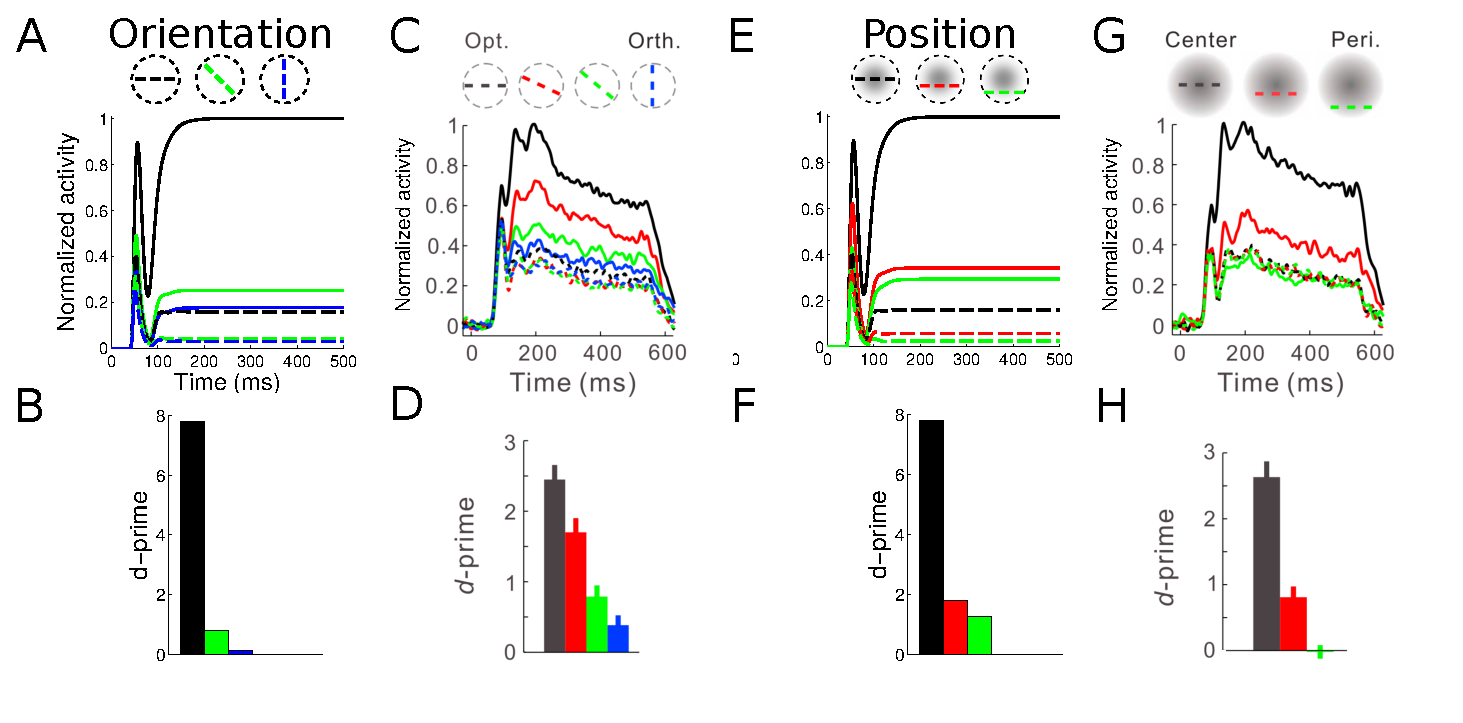
\includegraphics[width=\textwidth]{Contour/figs/FigS1.eps}
\end{center}
\makeatletter
\let\@currsize\normalsize
\caption[Orientation and position dependence of contour integration in V4]{Orientation and position dependence of contour integration in
  V4 $G_c$ cells. The top row shows neuronal responses and the bottom
  row the contour-response $d'$.  Line colors for each figure are
  indicated by the legends at the top of each column. Top row, solid
  lines indicate responses for the 7-bar contour pattern, while dashed
  lines indicate responses for the 1-bar noise pattern.  Note that
  orientations were changed in variable steps based on the tuning
  curve of the neuron under study in the experimental data
  (panels~C,~D) while our simulation only allowed steps of
  $\pi/4$ (panels~A,B).  (A and B) Model results, orientation
  dependence.
 The neuronal responses (A) and the contour-response $d'$
  (B) decreased when the contour was rotated away from the preferred
  orientation. (C and D) Analogous experimental results, adapted from
  \cite{Chen_etal14}.
  (E and F) Model
  results, position dependence.
 The neuronal responses (E) and
  contour-response $d'$ (F) decreased when the contour was translated away from the center of the V4 RF.
  (G and H) Analogous experimental results, adapted from \cite{Chen_etal14}. Panels C, D, G, and H are modified from Figure~3 of~\cite{Chen_etal14}.}
\label{Fig:V4_total}
\end{figure}

\begin{figure}[t]
\begin{center}
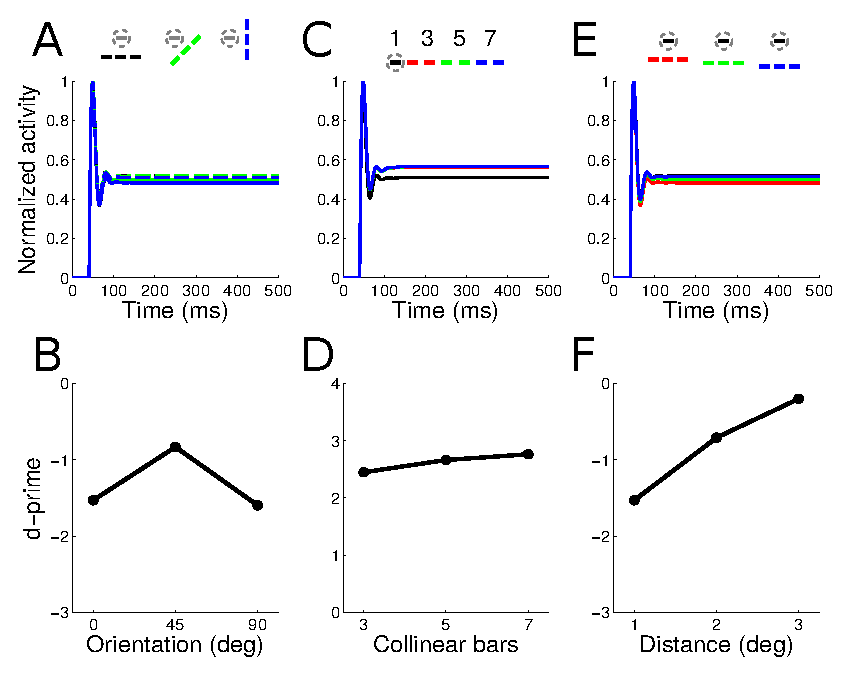
\includegraphics[width=\textwidth]{Contour/figs/FigS2.eps}
\end{center}
\makeatletter
\let\@currsize\normalsize
\caption[Orientation and position dependence of contour integration in V1]{Orientation and position dependence of contour integration in
  V1 $E$ cells, model results. The top row shows neuronal responses
  and the bottom row the contour-response $d'$. Line colors for each
  figures are indicated by the legends at the top of each column. (A
  and B) Orientation dependence of background suppression. The
  neuronal responses (A) and the contour-response $d'$ (B) increased
  for intermediate orientations of the background contour.
  In (A), solid and
  dashed lines correspond to the 7-bar contour and 1-bar noise patterns, respectively.
  (C and D) Contour integration on one end. The neuronal responses (C)
  and contour-response $d'$ (D) increased when bars were added to only
  one side of the V1 RF. (E and F) Position dependence of background
  suppression.  The neuronal responses (E) and contour-response $d'$ (F) increased (approached zero) when the background contour was moved away from the center of the V1 RF.}
\label{Fig:V1_total}
\end{figure}

%%% Local Variables:
%%% mode: latex
%%% TeX-master: "../root"
%%% End:
